\documentclass[11pt,a4paper]{article}

\usepackage[latin1]{inputenc} % encodage du fichier d'entr�e
\usepackage[T1]{fontenc} % encodage de la fonte
\usepackage{pgf}
\usepackage{classeRapport}
\usepackage{scrextend}
\usepackage{algorithme}
\usepackage{listings}
\usepackage{fixfoot}





\DeclareFixedFootnote{\repnote}{J'utilise un entier ici et non un
  naturel pour la position depuis le d�but de l'entr�e standard car
  cette position doit commencer � 0 donc j'initialise cette position �
  -1 dans le main}

\begin{document}
\PageDeGarde
{logo.png} % image sur la page de garde
{ASIspell} % titre principal
{Projet Correcteur Orthographique} % sous-titre
{Dounia \textsc{BOUTAYEB}\\ Thibault \textsc{SAURON}\\ Matthias
  \textsc{SESBO��}\\ Damien \textsc{TOOMEY}} % nom
{Algorithmique avanc�e et programmation C - ASI - 2017-2018} % bas de page

\Page{INSALogo}{logo.png} % logo de bas de page (en bas a droite)

\newpage
\tableofcontents

\newpage
\section{Introduction}
L'objectif de ce projet est de d�velopper un correcteur orthographique
efficace � l'image des programmes Unix ISPELL et Aspell. Le programme
doit d'une part, pouvoir analyser un texte qui lui est donn� via
l'entr�e standard et proposer des corrections orthographiques si
besoin. Cette analyse est d�pendante d'un dictionnaire qui contient au
d�part 336531 mots. Le programme doit d'autre part, donner la
possibilit� de compl�ter un dictionnaire � l'aide des mots d'un
fichier texte (un mot par ligne).

Nous avons �t� r�parti en groupe de quatre �tudiants. Ce projet permet
de nous mettre dans des conditions d'entreprise avec un chef de
projet, un d�lai et un cahier des charges � respecter. Le langage de
programmation impos� est le C. Nous devons utiliser la plateforme
monprojet pour faciliter l'�change du code.

\newpage
\section{R�sum� des s�ances}
\subsection{D�roulement du projet}

\begin{description}
\item[25/10/2017 : ] D�couverte du sujet et du
  groupe. \\Cr�ation du projet sur la plateforme
  \url{https://monprojet.insa-rouen.fr}.
  \\Conception de la premi�re
  version des TAD Mot,
  Dictionnaire et
  CorrecteurOrthograpique.

\item[08/11/2017 : ] Travail sur l'analyse descendante.

\item[15/11/2017 : ] Remise en cause des TAD.
  \\ Suppression de plusieurs fonctions et proc�dures
  non n�cessaires dans le cadre de notre projet. \\
  Ajouts et modifications de plusieurs fonctions et proc�dures.\\
  Le TAD Mot contient les op�rations permettant de faire
  toutes les modifications possibles sur un mot. \\
  Le TAD CorrecteurOrhtographique contient toutes les
  op�rations de correction. Ces op�rations sont en accord
  avec le fait que l'on traitera le texte � corriger
  comme un flux. On parcours le texte et on corrige mot
  par mot. On ne traite donc plus une liste de mots
  incorrectes.
  Choix de la structure de donn�e du type Dictionnaire. \\
  On choisit la structure de donn�e dynamique arbre N-aire, que
  l'on stockera � la mani�re d'un arbre binaire.

\item[22/11/2017 : ] Remise en cause de l'analyse descendante. \\
  Re-manipulation de l'analyse descendante, ajout de
  toutes les fonctions et proc�dures des TAD et
  suppression des proc�dures d'affichage. \\
  S�paration du travail pour la conception d�taill�e :
  \begin{itemize}
  \item[.] \emph{Damien} travaille sur les
    fonctions et proc�dures
    "queFaireEnFonctionDeCommandeDEntree",
    "afficherAide", ainsi que les fonctions et
    proc�dures du TAD
    "CorrecteurOrthographique".
  \item[.] \emph{Dounia} travaille sur les
    fonctions et proc�dures du TAD Mot.
  \item[.] \emph{Thibault} travaille sur les
    fonctions et proc�dures du TAD
    Dictionnaire.
  \item[.] \emph{Matthias} travaille avec \emph{Damien}
    sur les fonctions et proc�dures du TAD
    CorrecteurOrthographique, ainsi que sur le
    proc�dures "afficherMotBienEcrit",
    "afficherCorrectionsEtPosMot",
    "correctionDuMot" et "corrigerMot".
  \end{itemize}

\item[29/11/2017 : ] Analyse descendante finalis�e, conception
  d�taill�e en cours. S�paration du travail d'impl�mentation, �
  faire d�s que la conception d�taill�e est termin�e. \\
  S�paration du travail pour la conception d�taill�e :
  \begin{itemize}
  \item[.] \emph{Damien} d�veloppe les tests
    unitaires pour le TAD Mot (sauf celui de la
    fonction "obtenirMotEntreeStandard").
  \item[.] \emph{Dounia} d�veloppe les fonctions
    et proc�dures du TAD Ensemble.
  \item[.] \emph{Thibault} d�veloppe les tests
    unitaires pour le TAD
    CorrecteurOrhtographique ainsi que les
    fonctions et proc�dures du TAD
    Dictionnaire.
  \item[.] \emph{Matthias} d�veloppe les tests
    unitaires pour le TAD Dictionnaire et celui
    pour la fonction "obtenirMotEntreeStandard" ainsi que
    les fonctions et proc�dures du TAD
    CorrecteurOrthographique.
  \end{itemize}

\item[06/12/2017 : ] Nous continuons � d�velopper en C et
  ajout de quelques modifications. \\
  Modifications apport�es :
  \begin{itemize}
  \item[.] D�finition du SDD pour le type
    CorrecteurOrthographique : une structure
    contenant un Mot et un Dictionnaire. En
    cons�quence nous avons ajout� des fonctions
    accesseurs pour obtenir le Dictionnaire et le
    Mot.
  \item[.] D�finition du SDD pour le type
    Ensemble : une structure contenant deux
    champs, un pour les �l�ments et un autre pour le
    nombre d'�l�ments.
  \item[.] Nous avons choisi de d�velopper notre
    propre type ListeChaineeMot �tant donn� que
    nous n'utilisons qu'une liste cha�n�e de Mot
    et que nous n'avons besoin que de certaines
    fonctions et proc�dures.
  \end{itemize}
  S�paration du travail :
  \begin{itemize}
  \item[.] \emph{Damien} et \emph{Thibault}
    d�veloppent ensemble les TAD ArbreNaire et
    Dictionnaire.
  \item[.] \emph{Dounia} d�veloppe les TAD
    ListeChaineeMot et Mot.
  \item[.] \emph{Matthias} d�veloppe le TAD
    CorrecteurOrthographique.
  \end{itemize}

\item[13/12/2017 : ] Nous continuons � d�velopper en C. Suite
  � une mauvaise organisation de d�part, nous devons v�rifier
  les conventions de nommage pour nos codes soient coh�rents
  entre eux.\\
  S�paration du travail :
  \begin{itemize}
  \item[.] \emph{Damien} et \emph{Thibault}
    d�veloppent ensemble les proc�dures de
    s�rialisation et de d�s�rialisation.
  \item[.] \emph{Dounia} d�veloppe des tests unitaires.
  \item[.] \emph{Matthias} v�rifie que les
    conventions de nommage sont bien respect�es
    et travaille ensuite sur les tests
    unitaires.
  \end{itemize}

\item[20/12/2017 : ] Le d�veloppement de base est termin�, le
  code g�n�ral ainsi que les tests unitaires sont
  d�velopp�s. La s�ance consistait donc � faire passer les
  tests unitaires et donc commencer � corriger les code. \\
  Cette s�ance �tait la derni�re. L'objectif pour la fin de la
  semaine est de finir le code.
\end{description}

\subsection{Choix des conventions de nommage dans les .c et .h}

Une fois la conception d�taill�e termin�e, nous avons d� choisir des
conventions de nommage pour pouvoir d�velopper notre partie du code
chacun de notre c�t� tout en restant coh�rent avec le code des
autres.
Nous avons donc choisie les conventions suivantes :

\begin{description}
\item[TAD Mot : ] Nous adopterons les conventions suivantes :
  \begin{itemize}
  \item[.] Le type Mot sera nomm� : \emph{M\_Mot}.
  \item[.] Les fonctions et proc�dures du TAD
    Mot seront nomm�es de la fa�on suivante : \\
    \emph{M\_nomDeLaFonction ou M\_nomDeLaProc�dure}.
  \end{itemize}
\item[TAD Dictionnaire : ] Nous adopterons les conventions suivantes :
  \begin{itemize}
  \item[.] Le type Dictionnaire sera nomm� :
    \emph{D\_Dictionnaire}.
  \item[.] Les fonctions et proc�dures du TAD
    Dictionnaire seront nomm�es de la fa�on
    suivante : \\
    \emph{D\_nomDeLaFonction ou D\_nomDeLaProc�dure}.
  \end{itemize}
\item[TAD CorrecteurOrthographique : ] Nous adopterons les
  conventions suivantes :
  \begin{itemize}
  \item[.] Le type CorrecteurOrthographique sera
    nomm� :
    \emph{CO\_CorrecteurOrthographique}.
  \item[.] Les fonctions et proc�dures du TAD
    CorrecteurOrthographique seront nomm�es de
    la fa�on suivante : \\
    \emph{CO\_nomDeLaFonction ou CO\_nomDeLaProc�dure}.
  \end{itemize}
\item[TAD Ensemble : ] Nous adopterons les conventions suivantes :
  \begin{itemize}
  \item[.] Le type Ensemble sera nomm� :
    \emph{E\_Ensemble}.
  \item[.] Les fonctions et proc�dures du TAD
    Ensemble seront nomm�es de la fa�on suivante
    : \\
    \emph{E\_nomDeLaFonction ou E\_nomDeLaProc�dure}.
  \end{itemize}
\item[TAD ListeChaineeMot : ] Nous adopterons les conventions
  suivantes :
  \begin{itemize}
  \item[.] Le type ListeChaineeMot sera nomm� :
    \emph{LCM\_ListeChaineeMot}.
  \item[.] Les fonctions et proc�dures du TAD
    ListeChaineeMot seront nomm�es de la fa�on
    suivante : \\
    \emph{LCM\_nomDeLaFonction ou LCM\_nomDeLaProc�dure}.
  \end{itemize}
\item[TAD ArbreN : ] Nous adopterons les conventions suivantes :
  \begin{itemize}
  \item[.] Le type ArbreN sera nomm� : \emph{AbN\_ArbreN}.
  \item[.] Les fonctions et proc�dures du TAD
    ArbreN seront nomm�es de la fa�on suivante :
    \\
    \emph{AbN\_nomDeLaFonction ou Abn\_nomDeLaProc�dure}.
  \end{itemize}

\end{description}

\newpage
\section{Choix de la structure de donn�e du Dictionnaire}
\subsection{Choix possibles}

Nous allons ici discuter de trois choix possibles que nous avons pour
stocker les mots contenus dans le dictionnaire. Nous verrons les
avantages et les inconv�nients de ces diff�rentes structures de donn�e
et nous finirons par expliquer notre choix final.

\subsubsection{Tableau}

Nous pourrions, tr�s na�vement, choisir de stocker l'ensemble des mots
du dictionnaire dans un tableau. \\
Cette structure de donn�e statique aurait pour seul avantage un acc�s
aux mots en $\mathcal{O}$(1). \\
En revanche pour ce qui est de ses d�savantages ils sont nombreux :
\begin{itemize}
\item[.] Un tableau est une structure de donn�e statique. Or nous
  devons pouvoir ins�rer des mots facilement et donc faire varier la
  taille de ce tableau. Dans le cas pr�sent d'une structure de donn�e
  statique, nous devons choisir une taille maximum pour notre tableau
  � la compilation, ce qui n'est absolument pas int�ressant.
\item[.] L'insertion d'un nouveau mot va aussi poser probl�me
  puisqu'il faudra � chaque fois faire un d�calage de tous les mots
  qui sont situ�s apr�s l'indice d'insertion, avant d'ins�rer le
  mot.
\item[.] Un autre probl�me r�side dans la recherche d'un mot. En
  effet dans le cas d'un tableau, la recherche na�ve d'un mot sera en
  $\mathcal{O}$(n) o� n correspond au nombre de mot du dictionnaire, qui
  sera donc tr�s grand. Cette recherche ne sera par cons�quent
  absolument pas efficace. On pourrait l'am�liorer en faisant une
  recherche par dichotomie mais le fait que nous souhaitons stocker
  des mots rend sont utilisation impossible dans notre cas.
\end{itemize}

\subsubsection{Arbre binaire de recherche}

Nous pourrions choisir de stocker l'ensemble des mots � l'aide d'un
arbre binaire de recherche. \\
Cette structure de donn�e dynamique pr�sente deux gros avantages :

\begin{itemize}
\item[.] Un arbre binaire de recherche pr�sente des caract�ristiques
  particuli�res qui permettent la recherche d'un �l�ment en
  $\mathcal{O}$(log(n)) ce qui est tr�s int�ressant dans notre cas
  puisque nous allons devoir rechercher dans le dictionnaire si un mot
  existe, et ce avec une contrainte de temps.
\item[.] Cette structure de donn�e est dynamique. Ceci implique que
  nous pourrions faire varier la taille de notre arbre selon nos
  besoins au cours de l'ex�cution du programme, ce qui est un avantage
  important qui r�pond � un besoin de notre sujet.
\end{itemize}

Elle n�cessiterait en revanche de quantifier chaque mot avec une
valeur unique, ce qui reste faisable mais compliqu�, et de mettre en
place un moyen d'�quilibrer l'arbre afin d'avoir des temps de recherche correct.

\subsubsection{Arbre n-aire}

Enfin, nous pourrions choisir de stocker nos mots gr�ce � un arbre n-aire. \\

\begin{itemize}
\item[.] Cette structure de donn�e est aussi dynamique, en d�coule le
  m�me avantage que pour l'arbre binaire de recherche.
\item[.] L'arbre n-aire permettrait de stocker des lettres et non pas
  des mots. Ainsi, un mot devient un chemin de parcours de
  l'arbre. Par cons�quent la recherche d'un mot se fait en $\mathcal{O}$(n)
  o� n est le nombre de lettres maximal des mots. Ce qui donnerai un
  temps de recherche acceptable.
\item[.] Un avantage de cet arbre est la place qu'occupe la structure:
  comme les mots sont repr�sent�s par un chemin, on peut stocker par
  exemple 'abc' et 'ab' avec seulement 3 noeuds, ce qui permet d'avoir
  une structure de donn�e n�cessitant un espace m�moire relativement faible.
\end{itemize}



\subsubsection{Choix final}

Pour les raisons d'optimisation pr�sent�es pr�c�demment, nous ne
choisirons pas un tableau. Pour ce qui est des arbres le choix est
plus compliqu�. Les deux types d'arbres sont int�ressant et le choix
s'est fait sur la complexit� des algorithmes � d�velopper. En effet
dans le cas d'un arbre n-aire et dans celui d'un arbre binaire de
recherche le temps moyen de recherche est environ le m�me.
Dans l'arbre binaire de recherche, la hauteur d'un arbre est fonction
du nombre de mots alors que pour l'arbre n-aire elle est fonction du nombre
de lettres des mots. La hauteur maximum de celui-ci sera donc le nombre
de lettres du plus grand mot. Ce qui nous donne pour un arbre binaire
de recherche une taille de $\log_2(300000)=18.19$, soit une hauteur
maximale de 19, avec une partie importante des mots qui sera situ�e
sur les feuilles de par la construction de l'arbre.\\
Pour l'arbre n-aire, la taille maximale est plus grande
(anticonstitutionnellement fait 25 lettres) mais en moyenne en France
les mots font entre 6 et 7 caract�res suivant les sources, donc la
plupart des mots seront situ�s dans une hauteur de 7 environ. De plus
nous n'avons pas besoin de parcourir tout le tableau pour savoir si un
mot est mal orthographi�.\\
L� o� l'arbre binaire de recherche devient un peu moins int�ressant
c'est lorsqu'il s'agit d'ajouter (ou de supprimer) un mot dans le
dictionnaire. Dans la mesure o�, pour assurer la complexit� de
recherche d'un �l�ment en $\mathcal{O}$(log(n)), il faut s'assurer que
l'arbre reste �quilibr� en faisant des rotations apr�s chaque
insertion, cela implique des algorithmes plus compliqu�s; en tout cas
plus compliqu�s que pour l'arbre n-aire.
Les performances des deux arbres ayant l'air � peu pr�s �quivalente
nous choisirons celui qui sera plus simple � r�aliser : l'arbre n-aire.

\newpage
\section{Explication du Type Dictionnaire}
Notre dictionnaire est donc un arbre n-aire. Nous allons d�tailler son
utilisation.\\
Un arbre n-aire peut �tre visualis� comme un arbre binaire mais o�
seulement un seul fils fait 'descendre' dans la profondeur de l'arbre, on
parle de fils et de fr�re. comme dans l'exemple qui suit:

\begin{figure}[h]
  \centering
  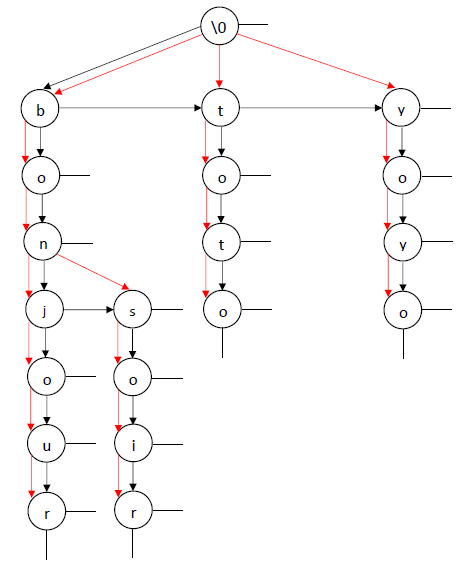
\includegraphics[width=10cm, height=12cm]{images/arbrenillustration.png}
  \caption{\label{�tiquette} Un exemple d'arbre n-aire}
\end{figure}

L�gende :
\begin{itemize}
\item[] Rouge : TAD Collection Arbre
\item[] Noir : Conception � l'aide d'un Arbre Binaire\\
\end{itemize}

Dans notre dictionnaire, la racine n'est pas utilis�e. Elle est ici pr�sente
car, par d�finition, la racine d'un arbre n-aire a un fr�re vide du
point de vue de la conception. Ici le 'a' est le fils de la racine et
le 't' est le fr�re de 'a'. L'int�r�t de cette repr�sentation est
qu'un mot devient un chemin de fils en fils et de fr�res en
fr�res. Pour savoir si un chemin est un mot valide, on rajoute un
champs � chaque noeud de notre arbre, une variable bool�enne
'motValide' par exemple. Sur la figure ci-dessus, si notre arbre
contient uniquement le mot 'yoyo', seulement le deuxi�me 'o' aura le
champ 'motValide' � VRAI car 'y', 'yo' et 'yoy' ne sont pas des mots
dans notre dictionnaire. Si on voulait ajouter le mot 'yoyos' il
suffirait d'ajouter le fils 's' au deuxi�me 'o' et d'avoir les champs
'motValide' � VRAI pour le deuxi�me 'o' et le 's'.

\newpage
\section{Analyse}
\subsection{Types Abstraits de Donn�es (TAD)}
\subsubsection{TAD Mot}

\begin{tad}
  \tadNom{Mot}
  \tadDependances{\caractere, \chaine, \naturelNonNul, \booleen, Ensemble}
  \begin{tadOperations}{}
    \tadOperation{longueur}{\tadUnParam{Mot}}{\tadUnParam{\naturel}}
    \tadOperationAvecPreconditions{obtenirIemeCaractere}{\tadDeuxParams{Mot}
      {\naturelNonNul}}{\tadUnParam{\caractere}}
    \tadOperationAvecPreconditions{fixerIemeCaractere}{\tadTroisParams{Mot}
      {\naturelNonNul}{\caractere}}{\tadUnParam{Mot}}
    \tadOperationAvecPreconditions{remplacerLettre}{\tadTroisParams{Mot}
      {\naturelNonNul}{\caractere}}{\tadUnParam{Mot}}
    \tadOperationAvecPreconditions{inverserDeuxLettresConsecutives}
    {\tadDeuxParams{Mot}{\naturelNonNul}}{\tadUnParam{Mot}}
    \tadOperationAvecPreconditions{supprimerLettre}{\tadDeuxParams{Mot}
      {\naturelNonNul}}{\tadUnParam{Mot}}
    \tadOperationAvecPreconditions{insererLettre}{\tadTroisParams{Mot}
      {\caractere}{\naturelNonNul}}{\tadUnParam{Mot}}
    \tadOperation{obtenirMotEntreeStandard}{\tadDeuxParams{Mot}{\entier \repnote}}
    {\tadTroisParams{\entier \repnote}{Mot}{\booleen}}
    \tadOperation{fixerLaChaine}{\tadDeuxParams{Mot}{\chaine}}{\tadUnParam{Mot}}
    \tadOperationAvecPreconditions{obtenirLaChaine}{\tadUnParam{Mot}}
    {\tadUnParam{\chaine}}
    \tadOperation{fixerLongueur}{\tadDeuxParams{Mot}{\naturel}}{\tadUnParam{Mot}}
    \tadOperation{obtenirLongueur}{\tadUnParam{Mot}}{\tadUnParam{\naturel}}
    \tadOperation{sontEgaux}{\tadDeuxParams{Mot}{Mot}}{\tadUnParam{\booleen}}
    \tadOperation{estUneLettre}{\tadUnParam{\caractere}}{\tadUnParam{\booleen}}
  \end{tadOperations}

  \begin{tadAxiomes}
    \tadAxiome{supprimer(insererLettre(mot, c, i), i)=mot}
    \tadAxiome{inverserDeuxLettresConsecutives(inverserDeuxLettresConsecutives(
      mot, pos), pos)=mot}
  \end{tadAxiomes}

  \begin{tadPreconditions}{}
    \tadPrecondition{obtenirIemeCaractere(mot, pos)}{1 $\leq$ pos
      $\leq$ obtenirLongueur(mot)}
    \tadPrecondition{fixerIemeCaractere(mot, pos, c)}{1 $\leq$ pos
      $\leq$ obtenirLongueur(mot)+1}
    \tadPrecondition{remplacerLettre(mot, pos, lettre)}{1 $\leq$ pos
      $\leq$ obtenirLongueur(mot)}
    \tadPrecondition{inverserDeuxLettresConsecutives(mot, pos)}{1
      $\leq$ pos $\leq$ obtenirLongueur(mot)-1}
    \tadPrecondition{supprimerLettre(mot, pos)}{(1 $\leq$ pos $\leq$
      obtenirLongueur(mot)) et (obtenirLongueur(mot) $\geq$ 2)}
    \tadPrecondition{insererLettre(mot, c, pos)}{1 $\leq$ pos $\leq$
      obtenirLongueur(mot)+1}
    \tadPrecondition{obtenirLaChaine(mot)}{obtenirLongueur(mot)>=0}
  \end{tadPreconditions}
\end{tad}

\subsubsection{TAD Dictionnaire}

\begin{tad}
  \tadNom{Dictionnaire}
  \tadParametres{Mot}
  \tadDependances{\booleen, \naturel}
  \begin{tadOperations}{}
    \tadOperation{creerDico}{}{\tadUnParam{Dictionnaire}}

    \tadOperation{estVide}{\tadUnParam{Dictionnaire}}{\tadUnParam{\booleen}}

    \tadOperation{insererMot}{\tadDeuxParams{Dictionnaire}{Mot}}
    {\tadUnParam{Dictionnaire}}

    \tadOperation{estPresent}{\tadDeuxParams{Dictionnaire}{Mot}}
    {\tadUnParam{\booleen}}

    \tadOperation{sauvegarderDico}{\tadDeuxParams{\chaine}{Dictionnaire}}
    {\tadUnParam{Fichier Texte}}

    \tadOperation{chargerDico}{\tadDeuxParams{\chaine}{Fichier Texte}}
    {\tadUnParam{Dictionnaire}}
  \end{tadOperations}

  \begin{tadAxiomes}
    \tadAxiome{insererMot(mot, insererMot(mot, dico))=insererMot(mot,dico)}

    \tadAxiome{estPresent(mot, insererMot(mot, dico)}
  \end{tadAxiomes}
\end{tad}

\subsubsection{TAD CorrecteurOrthographique}

\begin{tad}
  \tadNom{CorrecteurOrthographique}
  \tadParametres{Mot, Dictionnaire}
  \tadDependances{\booleen, Ensemble}
  \begin{tadOperations}{}
    \tadOperation{correcteurOrthographique}{}
    {\tadUnParam{CorrecteurOrthographique}}

    \tadOperationAvecPreconditions{proposerCorrection}
    {\tadDeuxParams{CorrecteurOrthographique}}{\tadUnParam{Ensemble<Mot>}}

    \tadOperationAvecPreconditions{estBienOrthographie}
    {\tadDeuxParams{CorrecteurOrthographique}}{\tadUnParam{\booleen}}

    \tadOperation{obtenirMot}{\tadUnParam{CorrecteurOrthographique}}
    {\tadUnParam{Mot}}

    \tadOperation{obtenirDictionnaire}{\tadUnParam{CorrecteurOrthographique}}
    {\tadUnParam{Dictionnaire}}

    \tadOperation{fixerMot}{\tadDeuxParams{CorrecteurOrthographique}{Mot}}
    {\tadUnParam{CorrecteurOrthographique}}

    \tadOperation{fixerDictionnaire}{\tadDeuxParams{CorrecteurOrthographique}
      {Dictionnaire}}{\tadUnParam{CorrecteurOrthographique}}
  \end{tadOperations}

  \begin{tadPreconditions}{}
    \tadPrecondition{proposerCorrection(co)}{non estBienOrthographie(co)}
  \end{tadPreconditions}
\end{tad}

\subsubsection{TAD Arbre n-aire}

Pour repr�senter notre TAD Dictionnaire nous avons choisis d'utiliser
un arbre n-aire. Nous allons maintenant d�tailler ce TAD.\\

\begin{tad}
  \tadNom{AbreN}
  \tadDependances{\booleen, \chaine, \caractere, Ensemble}
  \begin{tadOperations}{}

    \tadOperation{creerArbreNonInit}{}{\tadUnParam{ArbreN}}
    \tadOperation{estVide}{\tadUnParam{ArbreN}}{\tadUnParam{\booleen}}
    \tadOperationAvecPreconditions{obtenirBool}{\tadUnParam{ArbreN}}
    {\tadUnParam{\booleen}}
    \tadOperationAvecPreconditions{obtenirChar}{\tadUnParam{ArbreN}}
    {\tadUnParam{\caractere}}
    \tadOperationAvecPreconditions{fixerBool}{\tadDeuxParams{ArbreN}
      {\booleen}}{\tadUnParam{ArbreN}}
    \tadOperationAvecPreconditions{fixerChar}{\tadDeuxParams{ArbreN}
      {\caractere}}{\tadUnParam{ArbreN}}
    \tadOperationAvecPreconditions{fixerFils}{\tadDeuxParams{ArbreN}{ArbreN}}
    {\tadUnParam{ArbreN}}
    \tadOperationAvecPreconditions{fixerFrere}{\tadDeuxParams{ArbreN}{ArbreN}}
    {\tadUnParam{ArbreN}}
    \tadOperationAvecPreconditions{obtenirFils}{\tadUnParam{ArbreN}}
    {\tadUnParam{ArbreN}}
    \tadOperationAvecPreconditions{obtenirFrere}{\tadUnParam{ArbreN}}
    {\tadUnParam{ArbreN}}
  \end{tadOperations}

  \begin{tadPreconditions}{}

    \tadPrecondition{obtenirBool(arbre)}{non estVide(arbre)}
    \tadPrecondition{obtenirChar(arbre)}{non estVide(arbre)}
    \tadPrecondition{fixerBool(arbre, bool)}{non estVide(arbre)}
    \tadPrecondition{fixerChar(arbre, car)}{non estVide(arbre)}
    \tadPrecondition{fixerFils(arbre, fils)}{non estVide(arbre)}
    \tadPrecondition{fixerFrere(arbre, frere)}{non estVide(arbre)}
    \tadPrecondition{obtenirFils(arbre)}{non estVide(arbre)}
    \tadPrecondition{obtenirFrere(arbre)}{non estVide(arbre)}
  \end{tadPreconditions}
\end{tad}

\newpage
\subsection{Analyse descendante}

Notre analyse descendante se trouve sur les quatre pages suivantes. Du
fait de sa taille, les figures ne sont pas tr�s nettes. Nous vous
invitons donc � regarder les images AnalyseDescendanteMAIN-90,
AnalyseDescendanteMettreMotDansSDDdico-90, AnalyseDescendanteCorrigerMot-90,\\
AnalyseDescendanteobtenirMotEntreeStandard-90 au format jpg dans le
r�pertoire /rapport/images. Vous pouvez aussi cliquer
\href{https://drive.google.com/file/d/1KbCsgzSyPy5rJcjGTQRZmwdG7l1mG2OS/view?usp=sharing}{\emph{ici}},
pour voir, en ligne, l'image de l'analyse descendante du programme principale,
\href{https://drive.google.com/file/d/1I7NCatB1OX_qTifBynEafyC2xIsoMoRn/view?usp=sharing}{\emph{ici}}
pour celle correspondant � 'mettreMotDansSDDdico',
\href{https://drive.google.com/file/d/14eHbYWqVv2qjTY-rC_iW8tHbd5dhlxcR/view?usp=sharing}{\emph{ici}}
pour celle correspondant � `corrigerMot', ou encore
\href{https://drive.google.com/file/d/15DQ746vTvA2d2KU2f6ZqBqg-CSaY8RHV/view?usp=sharing}{\emph{ici}}
pour celle correspondant � 'obtenirMotEntreeStandard'.


\newpage
 \begin{center}
   \pgfimage[height=\textheight,interpolate=true]
   {images/AnalyseDescendanteMAIN-90}
 \end{center}

 \newpage
 \begin{center}
   \pgfimage[height=\textheight,interpolate=true]
   {images/AnalyseDescendanteobtenirMotEntreeStandard-90.jpg}
 \end{center}

 \newpage
 \begin{center}
   \pgfimage[height=\textheight,interpolate=true]
   {images/AnalyseDescendanteCorrigerMot-90.jpg}
 \end{center}

 \newpage
 \begin{center}
   \pgfimage[height=\textheight,interpolate=true]
   {images/AnalyseDescendanteMettreMotDansSDDdico-90.jpg}
 \end{center}

 \clearpage

\newpage
\section{Conception pr�liminaire}
\subsection{Signatures li�es au TAD Mot}
\begin{algorithme}

  \begin{enregistrement}{Mot}
    \champEnregistrement{laChaine}{\chaine}
    \champEnregistrement{longueur}{\naturel}
  \end{enregistrement}\\

  \signaturefonction {M.longueur}{mot : Mot}{\naturel}

  \signatureFonctionAvecPreconditions {M.obtenirIemeCaractere}{mot :
    Mot, pos : \naturelNonNul}{\caractere}{1 $\leq$ pos $\leq$
    M.obtenirLongueur(mot)}

  \signatureProcedureAvecPreconditions
  {M.fixerIemeCaractere}{\paramEntreeSortie{mot :
      Mot}, \paramEntree{pos : \naturelNonNul, lettre :\caractere}}{1
    $\leq$ pos $\leq$ M.obtenirLongueur(mot)+1}

  \signatureFonctionAvecPreconditions {M.remplacerLettre}{mot : Mot,
    pos : \naturelNonNul, lettre : \caractere}{Mot}{1 $\leq$ pos
    $\leq$ M.obtenirLongueur(mot)}

  \signatureFonctionAvecPreconditions
  {M.inverserDeuxLettresConsecutives}{mot : Mot, pos :
    \naturelNonNul}{Mot}{1 $\leq$ pos $\leq$ M.obtenirLongueur(mot)-1}

  \signatureFonctionAvecPreconditions {M.supprimerLettre}{mot : Mot,
    pos : \naturelNonNul}{Mot}{(1 $\leq$ pos $\leq$
    obtenirLongueur(mot)) et (obtenirLongueur(mot) $\geq$ 2)}

  \signatureFonctionAvecPreconditions {M.insererLettre}{mot : Mot, lettre :
    \caractere, pos : \naturelNonNul}{Mot}{1 $\leq$ pos $\leq$
    M.obtenirLongueur(mot)+1}

  \signatureprocedure
  {M.obtenirMotEntreeStandard}{\paramEntreeSortie{posDepuisDebutFlux :
      \entier \repnote, mot : Mot}, \paramSortie{arret :
      \booleen}}

  \signatureprocedure {M.fixerLaChaine}{\paramEntreeSortie{mot :
      Mot}, \paramEntree{chaine : \chaine}}

  \signatureFonctionAvecPreconditions {M.obtenirLaChaine}{mot :
    Mot}{\chaine}{M.obtenirLongueur(mot)>=0}

  \signatureprocedure {M.fixerLongueur}{\paramEntreeSortie{mot :
      Mot}, \paramEntree{length : \naturel}}

  \signaturefonction {M.obtenirLongueur}{mot : Mot}{\naturel}

  \signaturefonction {M.sontEgaux}{mot1, mot2 : Mot}{\booleen}

  \signaturefonction{M.estUneLettre}{c : \caractere}{\booleen}
\end{algorithme}

\subsection{Signatures li�es au TAD Dictionnaire}
\begin{algorithme}

  \type{Dictionnaire}{ArbreN}\\

  \signaturefonction {D.creerDico}{}{Dictionnaire}

  \signaturefonction {D.estVide}{dico : Dictionnaire}{\booleen}

  \signatureprocedure {D.insererMot}{\paramEntreeSortie{dico :
      Dictionnaire}, \paramEntree{lemot : Mot}}

  \signaturefonction {D.estPresent}{dico : Dictionnaire, mot : Mot}{\booleen}

  \signatureprocedure{D.sauvegarderDico}{\paramSortie{fichierSDDDico :
      Fichier Texte}, \paramEntree{dico : D.Dictionnaire}}

  \signatureFonctionAvecPreconditions{D.chargerDico}{nomFichier :
    \chaine, fichierSDDDico : Fichier
    Texte}{Dictionnaire}{F.fichierExiste(nomFichier)}
\end{algorithme}

\subsection{Signatures li�es au TAD CorrecteurOrthographique}

\begin{algorithme}

  \begin{enregistrement}{CorrecteurOrthographique}
    \champEnregistrement{mot}{Mot}
    \champEnregistrement{dico}{Dictionnaire}
  \end{enregistrement}\\

  \signaturefonction{CO.correcteurOrthographique}{}{CorrecteurOrthographique}

  \signatureFonctionAvecPreconditions {CO.proposerCorrection}{co :
    CorrecteurOrthographique}{Ensemble<Mot>}{non estBienOrthographie(co)}

  \signatureFonction {CO.estBienOrthographie}{co :
    CorrecteurOrthographique}{\booleen}

  \signatureFonction{CO.obtenirMot}{co : CorrecteurOrthographique}{Mot}
  \signatureFonction{CO.obtenirDictionnaire}{co :
    CorrecteurOrthographique}{Dictionnaire}

  \signatureprocedure{CO.fixerMot}{\paramEntreeSortie{co :
      CorrecteurOrthographique}, \paramEntree{mot : Mot}}

  \signatureprocedure{CO.fixerDictionnaire}{\paramEntreeSortie{co :
      CorrecteurOrthographique}, \paramEntree{dico : Dictionnaire}}
\end{algorithme}

\subsection{Signatures li�es au TAD Arbre n-aire}
\begin{algorithme}
  \type{ArbreN}{\typePointeur{Noeud}}

  \begin{enregistrement}{Noeud}
    \champEnregistrement{lettre}{\caractere}
    \champEnregistrement{motValide}{\booleen}
    \champEnregistrement{Fils}{ArbreN}
    \champEnregistrement{Frere}{ArbreN}
  \end{enregistrement}\\

  \signatureFonction {AbN.creerArbreNonInit}{}{ArbreN}

  \signatureFonction {AbN.estVide}{arbre : ArbreN}{\booleen}

  \signatureFonctionAvecPreconditions {AbN.obtenirBool}{arbre :
    ArbreN}{\booleen}{non AbN.estVide(arbre)}

  \signatureFonctionAvecPreconditions {AbN.obtenirChar}{arbre :
    ArbreN}{\caractere}{non AbN.estVide(arbre)}

  \signatureProcedureAvecPreconditions
  {AbN.fixerBool}{\paramEntreeSortie{arbre : ArbreN} \paramEntree{
      valide : \booleen}}{non AbN.estVide(arbre)}

  \signatureProcedureAvecPreconditions
  {AbN.fixerChar}{\paramEntreeSortie{arbre : ArbreN} \paramEntree{
      lalettre : \caractere}}{non AbN.estVide(arbre)}

  \signatureProcedureAvecPreconditions
  {AbN.fixerFils}{\paramEntreeSortie{arbre : ArbreN} \paramEntree{fils
      : ArbreN}}{non AbN.estVide(arbre)}

  \signatureProcedureAvecPreconditions
  {AbN.fixerFrere}{\paramEntreeSortie{arbre :
      ArbreN} \paramEntree{frere : ArbreN}}{non AbN.estVide(arbre)}

  \signatureFonctionAvecPreconditions {AbN.obtenirFils}{arbre :
    ArbreN}{ArbreN}{non AbN.estVide(arbre)}

  \signatureFonctionAvecPreconditions {AbN.obtenirFrere}{arbre :
    ArbreN}{ArbreN}{non AbN.estVide(arbre)}
\end{algorithme}

\subsection{Signatures des proc�dures d'affichage}
\begin{algorithme}
  \signatureprocedure {A.afficherAide}{}

  \signatureprocedure {A.affichageMotBienEcrit}{}

  \signatureprocedure
  {A.afficherCorrectionEtPosMot}{\paramEntree{lesCorrections :
      Ensemble<Mot>, leMot : Mot, pos : \naturel}}
\end{algorithme}

\subsection{Signatures des proc�dures priv�es du main}
\begin{algorithme}
  \signaturefonction{queFaireEnFonctionDeCommandeEntree \footnote{Nous ne
    mettons pas cette fonction en pseudocode dans la conception
    d�taill�e car elle est sp�cifique au langage utilis� (argc et agrv
    en C)}}{argc : \naturel, argv : tableau de CdC}{\naturelNonNul}

  \signatureprocedure{mettreMotsDansSDDdico}{\paramEntree{nomFichierSDDDico
      : \chaine, nomFichierTexteMotsAInserer : \chaine}}

  \signatureprocedure {corrigerMot}{\paramEntree{co :
      CorrecteurOrthographique, posMotFaux : \naturel}}
\end{algorithme}

\subsection{Signatures li�es au TAD Fichier Texte donn� dans le sujet}
\begin{algorithme}
  \signaturefonction{fichierTexte}{chaine : \chaine}{FichierTexte}

  \signatureProcedureAvecPreconditions{ouvrir}{\paramEntreeSortie{f :
      FichierTexte}, \paramEntree{Mode}}{non estOuvert(f)}

  \signatureProcedureAvecPreconditions{fermer}{\paramEntreeSortie{f :
      FichierTexte}}{estOuvert(f)}
  \signaturefonction{estOuvert}{f : FichierTexte}{Booleen}

  \signaturefonction{mode}{f : FichierTexte}{Mode}

  \signatureFonctionAvecPreconditions{finFichier}{f :
    FichierTexte}{Booleen}{mode(f)=lecture}

  \signatureProcedureAvecPreconditions{ecrireChaine}{\paramEntreeSortie{f
      : FichierTexte}, \paramEntree{chaine : \chaine}}{estOuvert(f) et
    mode(f)=ecriture}

  \signatureProcedureAvecPreconditions{lireChaine}{\paramEntreeSortie{f
      : FichierTexte}, \paramSortie{chaine : \chaine}}{estOuvert(f) et
    mode(f)=lecture et non finFichier(f)}

  \signatureProcedureAvecPreconditions{ecrireCaractere}{\paramEntreeSortie{f
      : FichierTexte}, \paramEntree{c : \caractere}}{estOuvert(f) et
    mode(f)=ecriture}

  \signatureProcedureAvecPreconditions{lireCaractere}{\paramEntreeSortie{f
      : FichierTexte}, \paramSortie{c : \caractere}}{estOuvert(f) et
    mode(f)=lecture et non finFichier(f)}
\end{algorithme}

\newpage
\section{Conception d�taill�e}
\subsection{Fonctions et proc�dures li�es au TAD Mot}

\subsubsection{Partie Priv�e}
\begin{algorithme}
  \constante{LETTRES\_SPECIALES\_AUTORISEES}
  {"��������������������������������������"}
  \constante{LONGUEUR\_LETTRES\_SPECIALES\_AUTORISEES}{38}
\end{algorithme} 

\subsubsection{Partie Publique}
\begin{algorithme}

  \begin{enregistrement}{Mot}
    \champEnregistrement{laChaine}{\chaine}
    \champEnregistrement{longueur}{\naturel}
  \end{enregistrement}\\

  \fonction {M.longueur}{mot : Mot}{\naturel}
  {}
  {
    \retourner{longueur(mot.laChaine)}
  }\\
  \fonction {M.obtenirLongueur}{mot : Mot}{\naturel}
  {}
  {
    \retourner{mot.longueur}
  }\\
  
\end{algorithme}

Nous pouvons remarquer ici que les deux derni�res fonctions semblent r�aliser la m�me action. Or dans le premier cas ("M.longueur") la fonction est une fonction d'encapsulation qui utilise la fonction "strlen" de la biblioth�que C "string.h". Nous l'utilisons une fois dans le code pour fixer la longueur du mot la premi�re fois. Ensuite nous ne nous servons plus que de l'accesseur "M.obtenirLongueur" qui renvoie le champ "longueur" de la structure Mot. En C, cet accesseur, nous permettra d'avoir acc�s � la longueur d'un mot en $\mathcal{O}$(1). \\

\begin{algorithme} 

  \fonctionAvecPreconditions{M.obtenirIemeCaractere}{mot : Mot, pos :
    \naturelNonNul}{Mot}{1 $\leq$ pos $\leq$ M.obtenirLongueur(mot)}
  {}
  {
    \retourner{mot[pos]}
  }\\

  \procedureAvecPreconditions{M.fixerIemeCaractere}{\paramEntreeSortie{mot
      : Mot}, \paramEntree{pos : \naturelNonNul, lettre :
      \caractere}}{1 $\leq$ pos $\leq$ M.obtenirLongueur(mot)+1}
  {}
  {
    \affecter{mot[pos]}{lettre}
  }\\

  \fonctionAvecPreconditions{M.remplacerLettre}{mot : Mot, pos :
    \naturelNonNul, lettre : \caractere}{Mot}{1 $\leq$ pos $\leq$
    M.obtenirLongueur(mot)}
  {}
  {
    \instruction{M.fixerIemeCaractere(mot, pos, lettre)}
    \retourner{mot}
  }\\

  \fonctionAvecPreconditions{M.inverserDeuxLettresConsecutives}{mot :
    Mot, pos : \naturelNonNul}{Mot}{1 $\leq$ pos $\leq$
    M.obtenirLongueur(mot)-1}
  {temp : \caractere}
  {
    \affecter{temp}{M.obtenirIemeCaractere(mot,pos)}
    \instruction {M.fixerIemeCaractere(mot, pos,
      M.obtenirIemeCaractere(mot,  pos+1))}
    \instruction {M.fixerIemeCaractere(mot, pos+1, temp)}
    \retourner{mot}
  }\\


  \fonctionAvecPreconditions{M.supprimerLettre}{mot : Mot, pos :
    \naturelNonNul}{Mot}{1 $\leq$ pos $\leq$ M.obtenirLongueur(mot)}
  {i : \naturelNonNul}
  {
    \pour{i}{pos}{M.obtenirLongueur(mot)}{}{
      \instruction{M.fixerIemeCaractere
        (mot, i, M.obtenirIemeCaractere(mot,i+1))}
    }
    \instruction{M.fixerLongueur(mot, M.obtenirLongueur(mot)-1)}
    \instruction{M.fixerIemeCaractere(mot, M.obtenirLongueur(mot),
      '\textbackslash 0')}
    \retourner{mot}
  }\\

  \fonctionAvecPreconditions{M.insererLettre}{mot : Mot, lettre :
    \caractere, pos : \naturelNonNul}{Mot}{1 $\leq$ pos $\leq$
    M.obtenirLongueur(mot)+1}
  {i : \naturelNonNul}
  {
    \pour{i}{longueur(mot)}{pos}{-1}{
      \instruction{M.fixerIemeCaractere(mot, i+1,
        M.obtenirIemeCaractere(mot, i))}
    }
    \instruction{M.fixerIemeCaractere(mot, pos, lettre)}
    \instruction{M.fixerLongueur(mot, M.obtenirLongueur(mot)+1)}
    \instruction{M.fixerIemeCaractere(mot, M.obtenirLongueur(mot),
      '\textbackslash 0')}
    \retourner{mot}
  }\\

  \fonction{M.estUneLettre}{c : \caractere}{\booleen}
  {{i : \naturelNonNul}\\
  {estPresent: \booleen}}
  {
    \affecter{i}{1}
    \affecter{estPresent}{FAUX}

    \tantque{(i<=LONGUEUR\_LETTRES\_SPECIALES\_AUTORISEES) et (estPresent=FAUX)}
    {

      \sialors {(LETTRES\_SPECIALES\_AUTORISEES[i]=c)} {
        \affecter{estPresent}{VRAI}
      }
      \affecter{i}{i+1}
    }
    \retourner{(estPresent ou ((c>='a') et (c<='z')) ou ((c>='A') et
      (c<='Z')) ou (c='-'))}
  }\\

  \procedure
  {M.obtenirMotEntreeStandard\footnote{Vous remarquerez que nous n'avons pas �crit de test unitaire pour cette proc�dure car nous ne savions pas comment faire. En effet, il aurait fallu ex�cuter le programme avec des param�tres au sein m�me du test unitaire. En revanche, nous avons test� cette proc�dure "� la main" dans de nombreux cas et elle passe nos tests}}{\paramEntreeSortie{posDepuisDebutFlux :
      \entier \repnote, mot : Mot}, \paramSortie{arret : \booleen}}
  {c : caractere}
  {

    \affecter{posDepuisDebutFlux}{posDepuisDebutFlux+naturelEnEntier(
      M.obtenirLongueur(mot))+1}
    \affecter{mot}{""}
    \affecter{c}{obtenirCaractereSuivantEntreeStandard()}

    \tantque{(non M.estUneLettre(c) et non estLaFinEntreeStandard(c))}{
      \affecter{c}{obtenirCaractereSuivantEntreeStandard()}
      \affecter{posDepuisDebutFlux}{posDepuisDebutFlux+1};
    }

    \tantque{M.estUneLettre(c) et non estLaFinEntreeStandard(c)}{
      \instruction{concatener(mot, majusculeEnMinuscule(caractereEnChaine(c)))}
      \affecter{c}{obtenirCaractereSuivantEntreeStandard()}
    }

    \instruction{fixerLongueur(mot, longueur(mot))}

    \sialors{estLaFinEntreeStandard(c)}{
      \affecter{arret}{VRAI}
    }
  }\\

  \procedure {M.fixerLaChaine}{\paramEntreeSortie{mot :
      Mot}, \paramEntree{chaine : \chaine}}
  {}
  {
    \affecter{mot.laChaine}{chaine}
  }\\

  \fonctionAvecPreconditions {M.obtenirLaChaine}{mot : Mot}{\chaine}
  {M.obtenirLongueur(mot)>=0}
  {}
  {
    \retourner{mot.laChaine}
  }\\

  \procedure {M.fixerLongueur}{\paramEntreeSortie{mot : Mot},
    \paramEntree{length : \naturel}}
  {}
  {
    \affecter{mot.longueur}{length}
  }\\

  \fonction {M.sontEgaux}{mot1, mot2 : Mot}{\booleen}
  {}
  {
    \retourner{M.obtenirLaChaine(mot1)=M.obtenirLaChaine(mot2)}
  }
  
\end{algorithme}

\subsection{Fonctions et proc�dures li�es au TAD Dictionnaire}

\subsubsection{Partie Priv�e}

\begin{algorithme}

  \constante{CaratereMotValide}{'*'}
  \constante{CaratereMotNonValide}{','}
  \constante{CaratereFilsNonVide}{'/'}
  \constante{CaratereFilsVide}{'.'}
  \constante{CaratereFrereNonVide}{':'}
  \constante{CaratereFrereVide}{';'}\\

  \procedure{serialiserParcoursRGDdico}{\paramEntree{dico :
      D.Dictionnaire}, \paramEntreeSortie{fichierSDDDico : Fichier Texte}}
  {}
  {

    \sialors{non D.estVide(dico)}{
      \instruction{ecrireCaractere(fichierSDDDico, AbN.obtenirChar(dico))}

      \sialorssinon{AbN.obtenirBool(dico)=VRAI}{
        \instruction{ecrireCaractere(fichierSDDDico, CaratereMotValide)}
      }
      {
        \instruction{ecrireCaractere(fichierSDDDico, CaratereMotNonValide)}
      }

      \sialorssinon{AbN.estVide(AbN.obtenirFils(dico))}{
        \instruction{ecrireCaractere(fichierSDDDico, CaratereFilsVide}
      }
      {
        \instruction{ecrireCaractere(fichierSDDDico, CaratereFilsNonVide)}
        \instruction{serialiserParcoursRGDdico(AbN.obtenirFils(dico),
          fichierSDDDico)}
      }

      \sialorssinon {AbN.estVide(AbN.obtenirFrere(dico))}{
        \instruction{ecrireCaractere(fichierSDDDico, CaratereFrereVide}
      }
      {
        \instruction{ecrireCaractere(fichierSDDDico, CaratereFrereNonVide)}
        \instruction{serialiserParcoursRGDdico(AbN.obtenirFrere(dico),
          fichierSDDDico)}
      }
    }
  }

  \procedure{deserialiser}{\paramEntreeSortie{dico :
      Dictionnaire}, \paramEntree{fichierSDDDico : Fichier Texte}}
  {{temp : Dictionnaire}\\
    {c : \caractere}}
  {
    \instruction{lireCaractere(fichierSDDDico, c)}
    \sialors {non finFichier(fichierSDDDico}{

      \instruction{AbN.fixerChar(dico, c)}

      \instruction{lireCaractere(fichierSDDDico, c)}

      \sialorssinon {c=CaratereMotValide} {
        \instruction{AbN.fixerBool(dico, VRAI)}
      }
      {
        \instruction{AbN.fixerBool(dico, FAUX)}
      }

      \instruction{lireCaractere(fichierSDDDico, c)}

      \sialors {c=CaratereFilsNonVide}{
        \affecter{temp}{D.creerDico()}
        \instruction{deserialiser(temp, fichierSDDDico)}
        \affecter{dico.Fils}{temp}
      }

      \instruction{lireCaractere(fichierSDDDico, c)}
      \sialors {c=CaratereFrereNonVide}{
        \affecter{temp}{D.creerDico()}
        \instruction{deserialiser(temp, fichierSDDDico)}
        \affecter{dico.Frere}{temp}
      }
    }
  }
\end{algorithme}

\subsubsection{Partie publique}

\begin{algorithme}
  \fonction {D.creerDico}{}{Dictionnaire}
  {dico : Dictionnaire}
  {
    \affecter{dico}{AbN.creerArbreNonInit()}
    \retourner{dico}
  }\\

  \fonction {D.estVide}{dico : Dictionnaire}{\booleen}
  {}
  {
    \retourner{AbN.estVide(dico)}
  }\\

  \procedure {D.insererMot}{\paramEntree{mot :
      Mot}, \paramEntreeSortie{dico : Dictionnaire}}
  {{temp, newNoeud, newNoeudTemp : Dictionnaire}\\
    {tempMot : Mot}}
  {
    \sialorssinon{D.estVide(dico)}{
      \affecter{dico}{D.creerDico()}
      \instruction{AbN.fixerChar(dico, M.obtenirIemeCaractere(tempMot,0))}
      \instruction{AbN.fixerBool(dico, M.obtenirLongueur(tempMot)=1)}

      \sialors{M.obtenirLongueur(tempMot)>1}{
        \affecter{temp}{AbN.obtenirFils(dico)}
        \instruction{D.insererMot(temp,M.supprimerLettre(tempMot,0))}
        \instruction{AbN.fixerFils(dico, temp)}
      }
    }
    {

      \sialorssinon{AbN.obtenirChar(dico) = M.obtenirIemeCaractere(tempMot,0)}{

        \sialorssinon{M.obtenirLongueur(tempMot) = 1}{
          \instruction{AbN.fixerBool (dico, VRAI)}
        }
        {
          \affecter{temp}{AbN.obtenirFils(dico)}
          \instruction{D.insererMot(temp,M.supprimerLettre(tempMot,0))}
          \instruction{AbN.fixerFils(dico, temp)}
        }

      }
      {
        \sialorssinon{AbN.obtenirChar(dico) <
          M.obtenirIemeCaractere(tempMot,0)} {
          \affecter{temp}{AbN.obtenirFrere(dico)}
          \instruction{D.insererMot(temp,tempMot)}
          \instruction{AbN.fixerFrere(dico, temp)}
        }
        {
          \affecter{temp}{dico}
          \affecter{newNoeud}{D.creerDico()}
          \instruction{AbN.fixerChar (newNoeud,
            M.obtenirIemeCaractere(tempMot,0))}
          \instruction{AbN.fixerBool (newNoeud, M.obtenirLongueur(tempMot)=1)}

          \sialorssinon{M.obtenirLongueur(tempMot)=1}{

            \instruction{AbN.fixerFrere(newNoeud, temp)}
            \instruction{AbN.fixerFils(newNoeud, newNoeudTemp)}
            \affecter{dico}{newNoeud}
          }
          {
            \affecter{newNoeudTemp}{AbN.obtenirFils(newNoeud)}
            \instruction{D.insererMot(newNoeudTemp,
              M.supprimerLettre(tempMot,0))
            }
            \instruction{AbN.fixerFrere(newNoeud, temp)}
            \instruction{AbN.fixerFils(newNoeud, newNoeudTemp)}
            \affecter{dico}{newNoeud}
          }
        }
      }
    }
  }\\

  \fonction {D.estPresent}{mot : Mot, dico : Dictionnaire}{\booleen}
  {temp : Mot}
  {
    \sialorssinon{D.estVide(dico)}{
      \retourner{FAUX}
    }
    {

      \sialorssinon{((M.obtenirLongueur(temp)=1) et
        (AbN.obtenirChar(dico) = M.obtenirIemeCaractere(temp,0)) et
        (AbN.obtenirBool(dico)=VRAI))}{
        \retourner{VRAI}
      }
      {

        \sialorssinon{((AbN.obtenirChar(dico) =
          M.obtenirIemeCaractere(temp,0) et (M.obtenirLongueur(temp)>1)))}{
          \retourner{D.estPresent(AbN.obtenirFils(dico),
            M.supprimerLettre(temp,0))}
        }
        {

          \sialorssinon {(AbN.obtenirChar(dico) <
            M.obtenirIemeCaractere(temp,0))}{
            \retourner{D.estPresent(AbN.obtenirFrere(dico),temp)}
          }
          {
            \retourner{FAUX}
          }
        }
      }
    }
  }\\

  \procedure{D.sauvegarderDico}{\paramSortie{fichierSDDDico : Fichier
      Texte}, \paramEntree{dico : D.Dictionnaire}}
  {}
  {
    \instruction{ouvrir(fichierSDDDico, ecriture)}
    \instruction{serialiserParcoursRGDdico(dico, fichierSDDDico)}
    \instruction{fermer(fichierSDDDico)}
  }

  \fonctionAvecPreconditions{D.chargerDico}{nomFichier : \chaine,
    fichierSDDDico : Fichier Texte}{Dictionnaire}{F.fichierExiste(nomFichier)}
  {dico : Dictionnaire}
  {
    \instruction{ouvrir(fichierSDDDico, lecture)}
    \affecter{dico}{D.creerDico()}
    \instruction{deserialiser(dico, fichierSDDDico)}
    \instruction{fermer(fichierSDDDico)}

    \retourner{dico}
  }

\end{algorithme}


\subsection{Fonctions et proc�dures li�es au TAD CorrecteurOrthographique}

\subsubsection{Partie priv�e}
\begin{algorithme}

  \constante{LETTRES\_SPECIALES\_AUTORISEES}
  {"��������������������������������������"}
  \constante{LONGUEUR\_LETTRES\_SPECIALES\_AUTORISEES}{38}\\

  \procedure {ajouterSiCorrecte}{\paramEntreeSortie{corrections :
      Ensemble<Mot>}, \paramEntree{co : CorrecteurOrthographique}}{}{
    \sialors{Co.estBienOrthographie(co)}
    {\instruction{E.ajouter(corrections, obtenirMot(co))}
    }
  }\\

\end{algorithme}

\subsubsection{Partie Publique}

\begin{algorithme}

  \fonctionAvecPreconditions {CO.proposerCorrection}{co :
    CorrecteurOrthographique}{Ensemble<Mot>}{non
    CO.estBienOrthographie(co)}
  {{i,k : \naturelNonNul}\\
    {j : \caractere}\\
    {temp, mot : Mot}\\
    {dico : Dictionnaire}\\
    {coTest : CorrecteurOrthographique}\\
    {corrections : Ensemble}}
  {
    \affecter{coTest}{CO.correcteurOrthographique()}
    \affecter{mot}{CO.obtenirMot(co)}
    \affecter{dico}{CO.obtenirDictionnaire(co)}
    \affecter{corrections}{E.ensemble()}

    \sialors{M.obtenirLongueur(mot)>=2}{
     \pour{i}{1}{M.obtenirLongueur(mot)}{}{
      \affecter{temp}{M.inverserDeuxLettreConsecutives(mot, i)}
      \instruction{CO.fixerMot(coTest,temp)}
      \instruction{ajouterSiCorrecte(corrections,coTest)}
     }
     \pour{i}{1}{M.obtenirLongueur(mot)+1}{}{
      \affecter{temp}{M.supprimerLettre(mot, i)}
      \instruction{CO.fixerMot(coTest,temp)}
      \instruction{ajouterSiCorrecte(corrections,coTest)}
     }
    }
    \pour{j}{'a'}{'z'}{}{
      \pour{i}{1}{M.obtenirLongueur(mot)}{}{
        \affecter{temp}{M.remplacerLettre(mot, i, j)}
        \instruction{CO.fixerMot(coTest,temp)}
        \instruction{ajouterSiCorrecte(corrections,coTest)}
      }
      }
      \tantque{k <= LONGUEUR\_LETTRES\_SPECIALES\_AUTORISEES}{
        \pour{i}{1}{M.obtenirLongueur(mot)+1}{}{
          \affecter{temp}{M.remplacerLettre(mot, i,
            LETTRES\_SPECIALES\_AUTORISEES[k])}
        \instruction{CO.fixerMot(coTest,temp)}
        \instruction{ajouterSiCorrecte(corrections,coTest)}
      }
      \instruction{k = k+1}
    }
     \pour{j}{'a'}{'z'}{}{
      \pour{i}{1}{M.obtenirLongueur(mot)+1}{}{
        \affecter{temp}{M.insererLettre(mot, j, i)}
        \instruction{CO.fixerMot(coTest,temp)}
        \instruction{ajouterSiCorrecte(corrections,coTest)}
      }
    }
     \tantque{k <= LONGUEUR\_LETTRES\_SPECIALES\_AUTORISEES}{
        \pour{i}{1}{M.obtenirLongueur(mot)+1}{}{
        \affecter{temp}{M.insererLettre(mot,
          LETTRES\_SPECIALES\_AUTORISEES[k], i)}
        \instruction{CO.fixerMot(coTest,temp)}
        \instruction{ajouterSiCorrecte(corrections,coTest)}
      }
      \instruction{k = k+1}
    }

    \retourner{corrections}
  }\\

  \fonction {CO.estBienOrthographie}{co : CorrecteurOrthographique}{\booleen}
  {}
  {
    \retourner{CO.estPresent(obtenirMot(co), CO.obtenirDictionnaire(co))}
  }\\

  \fonction{CO.obtenirMot}{co : CorrecteurOrthographique}{Mot}
  {}
  {
    \retourner{co.mot}
  }\\

  \fonction{CO.obtenirDictionnaire}{co : CorrecteurOrthographique}{Dictionnaire}
  {}
  {
    \retourner{co.dico}
  }\\

  \fonction{CO.correcteurOrthographique}{}{CorrecteurOrthographique}
  {{co : CorrecteurOrthographique}\\
    {mot : Mot}\\
    {dico : Dictionnaire}}
  {
    \instruction{M.fixerLaChaine(mot, "")}
    \instruction{M.fixerLongueur(mot, 0)}
    \instruction{CO.fixerMot(co, mot)}

    \affecter{dico}{NULL}
    \instruction{CO.fixerDictionnaire(co, dico)}

    \retourner{co}

  }

  \procedure{CO.fixerMot}{\paramEntreeSortie{co :
      CorrecteurOrthographique}, \paramEntree{mot : Mot}}
  {}
  {
    \affecter{co.mot}{mot}
  }

  \procedure{CO.fixerDictionnaire}{\paramEntreeSortie{co :
      CorrecteurOrthographique}, \paramEntree{dico : Dictionnaire}}
  {}
  {
    \affecter{co.dico}{dico}
  }

\end{algorithme}

\subsection{Fonctions et proc�dures li�es au TAD ArbreN}

\begin{algorithme}

  \fonction{AbN.creerArbreNonInit}{}{ArbreN}
  {temp:ArbreN}
  {
    \affecter{temp.Fils}{NULL}
    \affecter{temp.Frere}{NULL}
    \affecter{temp.lettre}{"caractereVide"}
    \affecter{temp.motValide}{0}
    \retourner{temp}
  }\\

  \fonction{AbN.estVide}{arbre :ArbreN}{\booleen}
  {}
  {
    \retourner{(arbre=NULL) ou (arbre.lettre="caractereNul")}
  }\\

  \fonctionAvecPreconditions{AbN.obtenirBool}{arbre :
    ArbreN}{\booleen}{non AbN.estVide(arbre)}
  {}
  {
    \retourner{(arbre.motValide)}
  }\\

  \fonctionAvecPreconditions{AbN.obtenirChar}{arbre :
    ArbreN}{\caractere}{non AbN.estVide(arbre)}
  {}
  {
    \retourner{(arbre.lettre)}
  }\\

  \procedureAvecPreconditions {AbN.fixerBool}{\paramEntreeSortie{arbre
      : ArbreN} \paramEntree{valide : \booleen}}{non AbN.estVide(arbre)}
  {}
  {
    \affecter{arbre.motValide}{valide}
  }

  \procedureAvecPreconditions {AbN.fixerChar}{\paramEntreeSortie{arbre
      : ArbreN} \paramEntree{ lalettre : \booleen}}{non AbN.estVide(arbre)}
  {}
  {
    \affecter{arbre.lettre}{lalettre}
  }

  \procedureAvecPreconditions {AbN.fixerFils}{\paramEntreeSortie{arbre
      : ArbreN} \paramEntree{fils : ArbreN}}{non AbN.estVide(arbre)}
  {}
  {

    \affecter{arbre.Fils}{fils}
  }

  \procedureAvecPreconditions
  {AbN.fixerFrere}{\paramEntreeSortie{arbre :
      ArbreN} \paramEntree{frere : ArbreN}}{non AbN.estVide(arbre)}
  {}
  {
    \affecter{arbre.Frere}{frere}
  }

  \fonctionAvecPreconditions{AbN.obtenirFils}{arbre :
    ArbreN}{ArbreN}{non AbN.estVide(arbre)}
  {}
  {
    \retourner{arbre.Fils}
  }\\

  \fonctionAvecPreconditions{AbN.obtenirFrere}{arbre :
    ArbreN}{ArbreN}{non AbN.estVide(arbre)}
  {}
  {
    \retourner{arbre.Frere}
  }\\

\end{algorithme}

\subsection{Proc�dures d'affichage}

\subsubsection{Partie priv�e}

\begin{algorithme}
  \constante{NOM\_FICHIER\_AIDE}{"./fichierAide.txt"}\\
\end{algorithme}

\subsubsection{Partie publique}

\begin{algorithme}
  \procedure
  {A.afficherCorrectionEtPosMot}{\paramEntree{lesCorrections :
      Ensemble<Mot>, leMot : Mot, pos : \naturel}}
  {{i, nbCorrections : \naturel}\\
    {mot : Mot}\\
    {lesMotsCorrects : ListeChaineeMot}}
  {
    \affecter{lesMotsCorrects}{E.obtenirLesElements(lesCorrections)}
    \affecter{nbCorrections}{E.cardinalite(lesCorrections)}

    \ecrire{"\&" M.obtenirLaChaine(leMot), naturelEnChaine(nbCorrections), naturelEnChaine(pos)}

    \pour{i}{0}{i<nbCorrections}{} {
      \affecter{mot}{LCM.obtenirElement(lesMotsCorrects)}
      \ecrire{M.obtenirLaChaine(mot)}
      \affecter{lesMotsCorrects}{LCM.obtenirListeSuivante(lesMotsCorrects)}
    }
  }\\

  \procedure {A.affichageMotBienEcrit}{}
  {}
  {
    \ecrire{"*"}
  }\\

  \procedure {A.afficherAide}{}
  {{fichierAide : Fichier Texte}\\
    {chaine : \chaine}}
  {
    \sialorssinon{F.fichierExiste(NOM\_FICHIER\_AIDE)} {
      \instruction{ouvrir(fichierAide, lecture)}
      \instruction{lireChaine(fichierAide, chaine)}
      \tantque {non finFichier(fichierAide)} {
        \ecrire{chaine}
      }
      \instruction{fermer(fichierAide)}
    }
    {
      \ecrire{"Le fichier d'aide est introuvable"}
    }
  }

\end{algorithme}

\subsection{Proc�dures priv�es du main}

\begin{algorithme}

    \procedure {corrigerMot}{\paramEntree{co : CorrecteurOrthographique,
      posMotFaux : \naturel}}
  {{correctionsPossibles : Ensemble}\\
  {temp : ListeChaineeMot}}
  {
    \affecter{correctionsPossibles}{ensemble()}

    \sialorssinon {non CO.estBienOrthographie(co)} {
      \affecter{correctionsPossibles}{CO.proposerCorrections(co)}
      \instruction{A.afficherCorrectionEtPosMot(correctionsPossibles,
        CO.obtenirMot(co), posMotFaux)}
    }
    {
      \instruction{A.affichageMotBienEcrit()}
    }
    \affecter{temp}{E.obtenirLesElements(correctionsPossibles)}
    \instruction{liberer(temp)}
  }\\

  \procedure{mettreMotsDansSDDdico}{(\paramEntree{nomFichierSDDDico :
      \chaine, fichierTexteMotsAInserer : Fichier Texte}}
  {{mot : Mot}\\
    {SDDDico, fils : Dictionnaire}\\
    {temp : \chaine}\\
    {longueurMot : \naturel}}
  {
    \affecter{SDDDico}{D.creerDico()}

    \sialorssinon {F.fichierExiste(nomFichierSDDDico)} {
      \affecter{SDDDico}{D.chargerDico(nomFichierSDDDico)}
      \instruction{AbN.fixerFils(SDDDico, fils)}
    }
    {
      \affecter{fils}{AbN.obtenirFils(SDDDico)}
    }

    \instruction{ouvrir(fichierTexteMotsAInserer, lecture)}

    \tantque {non finFichier(fichierTexteMotsAInserer)} {
      \instruction{lireChaine(fichierTexteMotsAInserer, temp)}
      \affecter{longueurMot}{longueur(temp)}
      \instruction{M.fixerLongueur(mot, longueurMot)}
      \instruction{M.fixerLaChaine(mot, temp)}

      \sialors {non D.estPresent(fils, mot)} {
        \instruction{D.insererMot(fils, mot)}
      }
    }
    \instruction{fermer(fichierTexteMotsAInserer)}

    \instruction{AbN.fixerFils(SDDDico, fils)}

    \instruction{D.sauvegarderDico(nomFichierSDDDico, fils)}
    \instruction{liberer(fils)}
    \instruction{liberer(SDDDico)}
  }

\end{algorithme}

\newpage
\section{Code C}
\lstset{language=C, numbers=left, morecomment = [l][\@gobble]{//}, morecomment = [is]{/*}{*/}}

\subsection{mot.h}
\lstinputlisting{../programme/include/mot.h}
\bigskip

\subsection{mot.c}
\lstinputlisting{../programme/src/mot.c}
\bigskip

\subsection{dictionnaire.h}
\lstinputlisting{../programme/include/dictionnaire.h}
\bigskip

\subsection{dictionnaire.c}
\lstinputlisting{../programme/src/dictionnaire.c}
\bigskip

\subsection{correcteurOrthographique.h}
\lstinputlisting{../programme/include/correcteurOrthographique.h}
\bigskip

\subsection{correcteurOrthographique.c}
\lstinputlisting{../programme/src/correcteurOrthographique.c}
\bigskip

\subsection{arbreN.h}
\lstinputlisting{../programme/include/arbreN.h}
\bigskip

\subsection{arbreN.c}
\lstinputlisting{../programme/src/arbreN.c}
\bigskip

\subsection{ensemble.h}
\lstinputlisting{../programme/include/ensemble.h}
\bigskip

\subsection{ensemble.c}
\lstinputlisting{../programme/src/ensemble.c}
\bigskip

\subsection{listeChaineeMot.h}
\lstinputlisting{../programme/include/listeChaineeMot.h}
\bigskip

\subsection{listeChaineeMot.c}
\lstinputlisting{../programme/src/listeChaineeMot.c}
\bigskip

\subsection{affichages.h}
\lstinputlisting{../programme/include/affichages.h}
\bigskip

\subsection{affichages.c}
\lstinputlisting{../programme/src/affichages.c}
\bigskip

\subsection{existeFichier.h}
\lstinputlisting{../programme/include/existeFichier.h}
\bigskip

\subsection{existeFichier.c}
\lstinputlisting{../programme/src/existeFichier.c}
\bigskip

\subsection{main.c}
\lstinputlisting{../programme/src/main.c}



\newpage
\section{Tests unitaires}
\lstset{language=C, numbers=left, morecomment = [l][\@gobble]{//}, morecomment = [is]{/*}{*/}}

\subsection{motTU.c}
\lstinputlisting{../programme/src/motTU.c}
\bigskip

\subsection{dictionnaireTU.c}
\lstinputlisting{../programme/src/dictionnaireTU.c}
\bigskip

\subsection{correcteurOrthographiqueTU.c}
\lstinputlisting{../programme/src/correcteurOrthographiqueTU.c}
\bigskip

\subsection{arbreNTU.c}
\lstinputlisting{../programme/src/arbreNTU.c}
\bigskip

\subsection{ensembleTU.c}
\lstinputlisting{../programme/src/ensembleTU.c}
\bigskip

\subsection{listeChaineeMotTU.c}
\lstinputlisting{../programme/src/listeChaineeMotTU.c}



\newpage
\section{Conclusion}
\subsection{Conclusion g�n�rale}
Ce projet �tait tr�s int�ressant. Le sujet du correcteur
orthographique est concret et permet de voir des aspects particuliers
d'un projet comme par exemple l'encodage des caract�res. Il nous a
ainsi permis d'apprendre le langage C, ainsi que le travail en �quipe
sur un probl�me informatique et dans des conditions r�elles de projet
en entreprise.\\
\indent
Nous sommes tout de m�me d��u car notre programme ne fonctionne qu'avec un dictionnaire sans accents (48843 mots) que nous avons trouv� sur internet (r�pertoire DicoSansAccents). Nous ne sommes pas parvenus � trouver le probl�me qui survient lorsque nous voulons construire notre SDD dictionnaire avec les mots du dictionnaire donn� sur Moodle. Nous avons cherch� et il nous semble que notre code est bon mais que nous avons des probl�mes avec l'encodage latin-1.\\
\indent
Nous avons tent� de trouver le probl�me avec Valgrind et ddd mais nous n'y sommes pas parvenus. Lorsqu'on utilise le dictionnaire avec accents, en mettant la commande suivante : valgrind \texttt{-{}-}leak-check=full \texttt{-{}-}track-origins=yes ./bin/asispell -d ./bin/francais.dico -f ./DicoAvecAccents/dico-ref-ascii.txt, Valgrind dit entre autres : Uninitialised value was created by a stack allocation at 0x10B1F5: D\_insererMot  (dictionnaire.c:130). Nous pensons donc que l'erreur survient dans D\_insererMot mais pas avec plus de pr�cision malheureusement.

\subsection{Conclusions personnelles}

\subsubsection{Dounia BOUTAYEB}
Ce projet s'est r�v�l� tr�s enrichissant dans la mesure o� il a
consist� en une approche concr�te du m�tier d'ing�nieur. En effet, la
prise d'initiative, le respect des d�lais et le travail en �quipe
seront des aspects essentiels de notre futur m�tier.
De plus, il nous a permis d'appliquer nos connaissances acquises en
cours et en travaux dirig�s et � utiliser le langage C. Ce qui m'a
aid� � mieux comprendre et � progresser.
Malgr� avoir eu quelques probl�mes au d�but avec l'utilisation de la
plateforme monprojet et TexMaker, j'ai pu m'investir dans le projet.

\subsubsection{Thibault SAURON}
J'ai beaucoup aim� travailler sur ce projet. Il m'a permis de me
mettre dans une situation concr�te de d�veloppement avec une �quipe,
un manager, des objectifs et une m�thode pr�cise. J'ai aussi pu
r�pondre � beaucoup de questions que je me posais sur le d�veloppement
d'un projet. Notamment le probl�me de gestion de versions que j'avais
rencontr� pendant le projet informatique en STPI2 ou produire
quelque chose de r�ellement utile et que je pourrais r�utiliser dans
des projets futurs. J'ai aussi pu me familiariser avec de nouveaux outils
comme \LaTeX\ et ddd qui me serons utiles plus tard.

\subsubsection{Matthias SESBO��}
Ce projet nous a permis de mettre en application ce que nous avons
appris tout au long du semestre de mani�re tr�s int�ressante. En plus
d'appliquer nos connaissances en programmation et en algorithmique, il
nous a aussi permis de d�couvrir ce que c'est de travailler en groupe
sur un projet informatique plus cons�quent que celui sur lequel nous
avions pu travailler en STPI. Enfin, nous avons d�couvert l'utilisation
du git, outil indispensable pour travailler sur une projet
informatique en �quipe.
En temps que chef de projet, j'ai beaucoup appr�ci� pouvoir "manager"
une �quipe dynamique constitu�e de personnes aux qualit�s et
comp�tences vari�es. Ces derni�res ont d'ailleurs entra�n� des
�changes int�ressants, qui ont abouti � des choix concrets et
efficaces en plus de permettre � chacun de progresser. Nous avons tous
travaill� de fa�on plus ou moins r�guli�re, avec chacun ses points
forts et ses points faibles. Malgr� quelques diff�rences de niveau et
d'investissement dans ce projet, je pense que nous nous sommes tous
investi et avons mis un maximum de volont� dans sa r�ussite.

\subsubsection{Damien TOOMEY}
Ce projet m'a permis d'apprendre � utiliser le langage C. Je me suis
rendu compte que le Pascal, enseign� en d�partement STPI, est une
�tape n�cessaire pour comprendre la base de la programmation car le C
est un langage plus compliqu� � manipuler. Ce projet m'a plu car
contrairement aux conditions d'un examen th�orique ou pratique, j'ai
pu y consacrer tout le temps que je voulais. L'utilisation de la
plateforme monprojet a facilit� le d�veloppement du code. En revanche,
je trouve que l'utilisation des demandes peut freiner la prise
d'initiatives.

\section{R�partition du travail}

\subsection{R�partition g�n�rale}
\begin{center}
  \begin{tabular}{ c c c c c }
    T�ches & BOUTAYEB & SAURON & SESBO�� & TOOMEY \\
           & Dounia & Thibault & Matthias & Damien \\
    TAD Mot & X & - & X & - \\
    TAD Dictionnaire & X & X & X & X \\
    partie priv�e Dictionnaire & - & - & - & X \\
    TAD CorrecteurOrthographique & - & - & X & - \\
    partie priv�e CO & - & - & X & - \\
    TAD arbre n-aire & - & X & - & - \\
    TAD ListeChaineeMot & X & - & - & - \\
    TAD Ensemble & - & - & X & - \\
    partie priv�e Ensemble & - & - & X & - \\
    programme principal & - & - & - & X \\
    proc�dures d'affichage & - & - & - & X \\
    ExisteFichier & - & - & - & X \\
    Tests unitaires TAD Mot & - & - & - & X \\
    Tests unitaires TAD Dictionnaire & - & X & - & - \\
    Tests unitaires TAD CO & - & X & X & X \\
    Tests unitaires TAD Arbre n-aire & - & X & - & - \\
    Tests unitaires TAD LCMot & - & - & - & X \\
    Tests unitaires TAD Ensemble & - & - & - & X \\
  \end{tabular}
\end{center}

\subsection{Travaux communs}

\begin{center}
  \begin{tabular}{ c c c c c }
    T�ches & BOUTAYEB & SAURON & SESBO�� & TOOMEY \\
           & Dounia & Thibault & Matthias & Damien \\
    Rapport & X & X & X & X \\
    Analyse descendante & X & X & X & X \\
    D.estPresent & - & - & X & - \\
    D.insererMot & - & - & X & X \\
  \end{tabular}
\end{center}

\end{document}